% Options for packages loaded elsewhere
\PassOptionsToPackage{unicode}{hyperref}
\PassOptionsToPackage{hyphens}{url}
\PassOptionsToPackage{dvipsnames,svgnames,x11names}{xcolor}
%
\documentclass[
  letterpaper,
  DIV=11,
  numbers=noendperiod]{scrartcl}

\usepackage{amsmath,amssymb}
\usepackage{iftex}
\ifPDFTeX
  \usepackage[T1]{fontenc}
  \usepackage[utf8]{inputenc}
  \usepackage{textcomp} % provide euro and other symbols
\else % if luatex or xetex
  \usepackage{unicode-math}
  \defaultfontfeatures{Scale=MatchLowercase}
  \defaultfontfeatures[\rmfamily]{Ligatures=TeX,Scale=1}
\fi
\usepackage{lmodern}
\ifPDFTeX\else  
    % xetex/luatex font selection
\fi
% Use upquote if available, for straight quotes in verbatim environments
\IfFileExists{upquote.sty}{\usepackage{upquote}}{}
\IfFileExists{microtype.sty}{% use microtype if available
  \usepackage[]{microtype}
  \UseMicrotypeSet[protrusion]{basicmath} % disable protrusion for tt fonts
}{}
\makeatletter
\@ifundefined{KOMAClassName}{% if non-KOMA class
  \IfFileExists{parskip.sty}{%
    \usepackage{parskip}
  }{% else
    \setlength{\parindent}{0pt}
    \setlength{\parskip}{6pt plus 2pt minus 1pt}}
}{% if KOMA class
  \KOMAoptions{parskip=half}}
\makeatother
\usepackage{xcolor}
\setlength{\emergencystretch}{3em} % prevent overfull lines
\setcounter{secnumdepth}{-\maxdimen} % remove section numbering
% Make \paragraph and \subparagraph free-standing
\makeatletter
\ifx\paragraph\undefined\else
  \let\oldparagraph\paragraph
  \renewcommand{\paragraph}{
    \@ifstar
      \xxxParagraphStar
      \xxxParagraphNoStar
  }
  \newcommand{\xxxParagraphStar}[1]{\oldparagraph*{#1}\mbox{}}
  \newcommand{\xxxParagraphNoStar}[1]{\oldparagraph{#1}\mbox{}}
\fi
\ifx\subparagraph\undefined\else
  \let\oldsubparagraph\subparagraph
  \renewcommand{\subparagraph}{
    \@ifstar
      \xxxSubParagraphStar
      \xxxSubParagraphNoStar
  }
  \newcommand{\xxxSubParagraphStar}[1]{\oldsubparagraph*{#1}\mbox{}}
  \newcommand{\xxxSubParagraphNoStar}[1]{\oldsubparagraph{#1}\mbox{}}
\fi
\makeatother


\providecommand{\tightlist}{%
  \setlength{\itemsep}{0pt}\setlength{\parskip}{0pt}}\usepackage{longtable,booktabs,array}
\usepackage{calc} % for calculating minipage widths
% Correct order of tables after \paragraph or \subparagraph
\usepackage{etoolbox}
\makeatletter
\patchcmd\longtable{\par}{\if@noskipsec\mbox{}\fi\par}{}{}
\makeatother
% Allow footnotes in longtable head/foot
\IfFileExists{footnotehyper.sty}{\usepackage{footnotehyper}}{\usepackage{footnote}}
\makesavenoteenv{longtable}
\usepackage{graphicx}
\makeatletter
\newsavebox\pandoc@box
\newcommand*\pandocbounded[1]{% scales image to fit in text height/width
  \sbox\pandoc@box{#1}%
  \Gscale@div\@tempa{\textheight}{\dimexpr\ht\pandoc@box+\dp\pandoc@box\relax}%
  \Gscale@div\@tempb{\linewidth}{\wd\pandoc@box}%
  \ifdim\@tempb\p@<\@tempa\p@\let\@tempa\@tempb\fi% select the smaller of both
  \ifdim\@tempa\p@<\p@\scalebox{\@tempa}{\usebox\pandoc@box}%
  \else\usebox{\pandoc@box}%
  \fi%
}
% Set default figure placement to htbp
\def\fps@figure{htbp}
\makeatother
% definitions for citeproc citations
\NewDocumentCommand\citeproctext{}{}
\NewDocumentCommand\citeproc{mm}{%
  \begingroup\def\citeproctext{#2}\cite{#1}\endgroup}
\makeatletter
 % allow citations to break across lines
 \let\@cite@ofmt\@firstofone
 % avoid brackets around text for \cite:
 \def\@biblabel#1{}
 \def\@cite#1#2{{#1\if@tempswa , #2\fi}}
\makeatother
\newlength{\cslhangindent}
\setlength{\cslhangindent}{1.5em}
\newlength{\csllabelwidth}
\setlength{\csllabelwidth}{3em}
\newenvironment{CSLReferences}[2] % #1 hanging-indent, #2 entry-spacing
 {\begin{list}{}{%
  \setlength{\itemindent}{0pt}
  \setlength{\leftmargin}{0pt}
  \setlength{\parsep}{0pt}
  % turn on hanging indent if param 1 is 1
  \ifodd #1
   \setlength{\leftmargin}{\cslhangindent}
   \setlength{\itemindent}{-1\cslhangindent}
  \fi
  % set entry spacing
  \setlength{\itemsep}{#2\baselineskip}}}
 {\end{list}}
\usepackage{calc}
\newcommand{\CSLBlock}[1]{\hfill\break\parbox[t]{\linewidth}{\strut\ignorespaces#1\strut}}
\newcommand{\CSLLeftMargin}[1]{\parbox[t]{\csllabelwidth}{\strut#1\strut}}
\newcommand{\CSLRightInline}[1]{\parbox[t]{\linewidth - \csllabelwidth}{\strut#1\strut}}
\newcommand{\CSLIndent}[1]{\hspace{\cslhangindent}#1}

\usepackage{booktabs}
\usepackage{longtable}
\usepackage{array}
\usepackage{multirow}
\usepackage{wrapfig}
\usepackage{float}
\usepackage{colortbl}
\usepackage{pdflscape}
\usepackage{tabu}
\usepackage{threeparttable}
\usepackage{threeparttablex}
\usepackage[normalem]{ulem}
\usepackage{makecell}
\usepackage{xcolor}
\usepackage{caption}
\usepackage{anyfontsize}
\usepackage{lineno}\linenumbers
\KOMAoption{captions}{tableheading}
\makeatletter
\@ifpackageloaded{caption}{}{\usepackage{caption}}
\AtBeginDocument{%
\ifdefined\contentsname
  \renewcommand*\contentsname{Table of contents}
\else
  \newcommand\contentsname{Table of contents}
\fi
\ifdefined\listfigurename
  \renewcommand*\listfigurename{List of Figures}
\else
  \newcommand\listfigurename{List of Figures}
\fi
\ifdefined\listtablename
  \renewcommand*\listtablename{List of Tables}
\else
  \newcommand\listtablename{List of Tables}
\fi
\ifdefined\figurename
  \renewcommand*\figurename{Figure}
\else
  \newcommand\figurename{Figure}
\fi
\ifdefined\tablename
  \renewcommand*\tablename{Table}
\else
  \newcommand\tablename{Table}
\fi
}
\@ifpackageloaded{float}{}{\usepackage{float}}
\floatstyle{ruled}
\@ifundefined{c@chapter}{\newfloat{codelisting}{h}{lop}}{\newfloat{codelisting}{h}{lop}[chapter]}
\floatname{codelisting}{Listing}
\newcommand*\listoflistings{\listof{codelisting}{List of Listings}}
\makeatother
\makeatletter
\makeatother
\makeatletter
\@ifpackageloaded{caption}{}{\usepackage{caption}}
\@ifpackageloaded{subcaption}{}{\usepackage{subcaption}}
\makeatother

\usepackage{bookmark}

\IfFileExists{xurl.sty}{\usepackage{xurl}}{} % add URL line breaks if available
\urlstyle{same} % disable monospaced font for URLs
\hypersetup{
  pdftitle={Measuring children's early vocabulary in low-resource languages using a Swadesh-style word list},
  pdfkeywords={early language learning; Communicative Development
Inventory; psychometrics; cross-linguistic comparison; vocabulary},
  colorlinks=true,
  linkcolor={blue},
  filecolor={Maroon},
  citecolor={Blue},
  urlcolor={Blue},
  pdfcreator={LaTeX via pandoc}}


\title{Measuring children's early vocabulary in low-resource languages
using a Swadesh-style word list}
\author{George Kachergis* \and Alvin Wei Ming Tan* \and Virginia A.
Marchman \and Philip S. Dale \and Michael C. Frank}
\date{}

\begin{document}
\maketitle
\begin{abstract}
Early language skill is predictive of many later life outcomes, and is
thus of great interest to developmental psychologists and clinicians.
The MacArthur-Bates Communicative Development Inventories (CDIs), parent
report instruments typically containing inventories of hundreds of
children's vocabulary words, have proven to be valid and reliable
instruments for measuring children's early language skill. The CDIs have
been adapted to many dozens of languages, and cross-linguistic
comparisons show both consistency and variability in language
acquisition trajectories. However, thousands of languages do not yet
have CDIs, nor the early language corpora needed to create them, posing
a significant barrier to increasing the diversity of languages that are
studied. Here, we propose a method for selecting candidate words to
include on new CDIs through analyzing psychometric properties of the
translation-equivalent concepts that are frequently included on existing
CDIs. Leveraging 32 datasets from existing CDIs, we propose a list of
100 concepts that have low variability in their cross-linguistic
learning difficulty. This pool of common concepts---analogous to the
Swadesh lists, which are basic vocabulary lists used in glottochronology
for cross-language comparison---can be used as a starting point for
future CDI adaptations. We show that the proposed Swadesh-CDI list
generalizes well to data from 10 additional languages.
\end{abstract}


\section{Introduction}\label{introduction}

Tools that enable valid assessments of children's early language
abilities are invaluable for researchers, clinicians and parents, as
early language skill is predictive of educational outcomes years later
(e.g., Bleses et al. 2016). The MacArthur-Bates Communicative
Development Inventories (CDIs; Fenson et al. 2007; Marchman, Dale, and
Fenson 2023) are parent report assessments that provide reliable and
valid estimates of children's early vocabulary size and other aspects of
early communicative development, such as use of gestures and of word
combinations. Parent report is a relatively quick and low-cost method to
assess early language skills as it takes advantage of the fact that
parents are ``natural observers'' of their child's skills and it does
not depend on a child engaging with an unfamiliar experimenter.

Over the years, the CDIs have been adapted to dozens of languages, with
forms now available in English, Spanish, French, Hebrew, and Mandarin,
to name just a few. At present, data from 97,925 CDIs in 42 languages
have been archived in a central, open repository (Wordbank, Frank et al.
2017). Analyses of these data have revealed both cross-linguistic
consistency and variability in early language skills, with insights from
these patterns informing theories of early language learning (Frank et
al. 2021). For example, cross-linguistic analyses indicate that measures
of vocabulary size are tightly correlated with other aspects of early
language skill, such as gesture and grammatical competence. Thus, over
development, the language system is ``tightly woven'' (Bates et al.
1994; Frank et al. 2021) and early vocabulary size serves as a good
proxy measure of children's overall language skill.

On the CDIs, vocabulary size is assessed via a checklist format, which
enables caregivers to scan and recognize words their child produces or
understands, rather than relying on recall alone. For example, the
American English CDI Words \& Sentences (CDI:WS) form, targeting
children 16--30 months of age, is composed of 680 words from 22 semantic
categories, including nouns (e.g., body parts, toys, clothing), action
words, descriptive words, and closed-class words, such as pronouns.
Items on this original CDI:WS were chosen to reflect a range of
difficulty levels (i.e., easy, moderate, and more difficult), as well as
capture the linguistic and societal contexts of (most) children living
in the US. The American English CDI Words \& Gestures form (CDI:WG)
targets children 8--18 months of age, consisting of approximately 400
items that include some of the easier items from the CDI:WS. This form
asks caregivers to report on children's comprehension (``understands'')
as well as their production (``understands and says'') of each word.
Short versions of the CDI:WG and CDI:WS forms are also available (e.g.,
Marchman, Dale, and Fenson 2023), each consisting of a set of around 100
items. The words on the short forms were selected such that scores
strongly correlate with scores on the full forms, while retaining
representation across a broad set of semantic categories.

Adapting a new CDI requires substantial effort and resources. Following
the guidelines from the MacArthur-Bates CDI Advisory Board\footnote{The
  adaptation guidelines can be found at
  \url{https://mb-cdi.stanford.edu/adaptations.html}.}, the process of
adapting a CDI for a language other than American English goes well
beyond simply translating items on these forms to that new language (see
Jarůšková et al. 2023; Brookes et al. 2025). The process can begin with
identifying translation equivalents (i.e., items that capture the same
general concept in both languages, e.g., ``dog'' in English, and
``perro'' in Spanish), but the final item set must then be filtered so
that all items appropriately reflect the linguistic and sociocultural
context of the children learning that language. This process requires
considerable time and effort by researchers who are both native speakers
of the language and who have experience with children, first to select
and identify translation equivalents and then to iteratively add,
refine, and pilot the new CDI in the target language. Because the goal
is to obtain the set of items that best capture general trends and
individual differences in that language, the items across CDIs in
different languages do not necessarily overlap to a great extent. For
example, the American English CDI:WS and Mexican Spanish CDI:WS forms
each have 680 words, but only have 463 overlapping concepts (68\%).

While CDI adaptations now exist for many languages, there remain
important gaps in language coverage. For example, the CDIs have been
adapted to very few languages in India and Africa, despite the large
number of speakers of some of these overlooked languages (e.g., Punjabi,
Marathi, Telugu, Hausa, and Amharic, all of which have over 50 million
speakers; see Eberhard, Simons, and Fennig 2025). Moreover, the CDIs
have not been adapted to almost all of the thousands of languages spoken
by indigenous peoples around the world. The dearth of CDIs in these
languages is a significant barrier to understanding the diversity of
language development across the world, which is crucial for developing
and validating theories of language acquisition that are purportedly
universal (Kidd and Garcia 2022; Singh et al. 2023). More broadly, the
research and clinical communities speaking these languages are often
under-resourced and may lack a language resource ecosystem which would
provide not only vocabulary assessment instruments, but also corpora,
acquisition descriptions, computational tools, and other resources that
support language development research and clinical practice (Hellwig et
al. 2021). The absence of these resources also makes adaptations of the
CDIs more difficult. For example, examining corpora of child and
child-directed language is a common method for selecting items for a new
CDI (Jarůšková et al. 2023) and this approach would not be possible if
such corpora do not exist, or are not appropriately pre-processed and
made accessible.

The importance and challenge of adapting the CDI to new, low-resource
languages prompts the following question: Can we find a less
resource-intensive way to create new CDIs that are valid and reliable?
One possible approach is to identify a small set of items that are
learned consistently across many languages, and which would meet the
criteria for inclusion on many CDIs. This approach would lower the
burden of creating CDIs in new languages, as a translation of this
common set of items could serve as the basis for a new CDI adaptation.
Furthermore, finding a small set of items that are nonetheless highly
informative for vocabulary assessment could also lead to shorter
assessments in languages that already have CDIs.

Our goal in the current study is to leverage the roughly 100,000 CDI
administrations from 32 languages on Wordbank to choose and
systematically evaluate small sets of items that may meet researchers'
criteria for creating a new CDI. To facilitate this effort, item
response theory (IRT; Embretson and Reise 2013) models are useful, as
they infer both the abilities of test takers and the difficulty of
individual test items (i.e., words), along standardized dimensions.
Recent work using IRT models has facilitated our understanding of the
psychometric properties of specific CDI instruments. As such, they offer
the potential to not only yield more accurate measures of children's
language ability, but also to enable the construction of
language-specific computerized adaptive tests (CATs), which iteratively
choose the next test item based on the responses to the previous items,
and thus quickly home in on the test taker's language ability. CAT-based
CDIs presenting 50 or fewer items have been found to strongly correlate
with scores on the full CDI:WS (Chai, Lo, and Mayor 2020; Mayor and Mani
2019; Makransky et al. 2016). A general method for creating CDI CATs
that works well across a broader age range (12--36 months) has been
proposed and tested for American English and Mexican Spanish (Kachergis
et al. 2022). Note that the IRT model driving each CAT needs to be
trained on a large and normative dataset (that is, a sample that is
representative of a target population), which may not be available in a
given language. To date, the IRT models are fitted separately for each
language and the fitted parameters (e.g., word difficulty) are likely to
vary across languages. Notably, this work has also revealed that scores
on random subsets of items from a CDI form are highly correlated with
scores on the full CDI (e.g., for English, full CDI vs.~100 random items
\(r=0.989\); Kachergis et al. 2022), making random selection an
important baseline comparison for any other proposed method. However,
random items from a single form are not guaranteed to be (1)
developmentally and culturally appropriate in other languages, (2) of
similar difficulty in other languages, or (3) representative of the
semantic or syntactic categories on the full CDI.

The goal of the current study is to use IRT modeling in conjunction with
data from Wordbank to examine whether there is a core set of concepts
that are frequently included on CDIs, and---importantly---whether enough
of them are of roughly equal difficulty across many languages to allow
them to be used as candidate items in new CDI adaptations. This work
takes its inspiration from the fields of lexicostatistics and
glottochronology, where researchers (notably, Swadesh 1971) have
proposed lists of common concepts that exist in all catalogued languages
in order to quantify the genealogical relatedness and dates of
divergence of languages. The original Swadesh list contains 100 words,
comprised of categories including common pronouns (``I'', ``you'',
``we''), animals (``man'', ``fish'', ``bird'', ``dog''), objects
(``tree'', ``leaf'', ``sun'', ``mountain''), and verbs (``die'',
``see'', ``sleep'', ``kill''). Extending this work to the development of
a universal CDI, or ``Swadesh CDI'', would involve (a) identifying those
concepts that researchers have chosen to include on CDI adaptations, (b)
determining the relative difficulty of those items across languages, and
(c) identifying those items with the least cross-linguistic variation.
If such a list of words were identified, it could serve as a helpful
starting point for the development of new CDI adaptations. The
constituent words already have good estimates of cross-linguistic
difficulty, providing a method to approximate children's language
abilities in the absence of a sufficiently-large norming study.

Our contributions are to (1) revise and extend a set of
translation-equivalent concepts in Wordbank, (2) fit IRT models to
CDI:WG and CDI:WS data from 32 languages, (3) evaluate candidate lists
of Swadesh CDI (S-CDI) items from a cross-linguistic comparison of
concept difficulty and inclusion, (4) identify and characterize the most
consistent 100 items to compose a S-CDI list, and (5) evaluate its
generalization to a set of 10 additional low-data languages. We then
make a concrete proposal for how this S-CDI list could be used to create
future CDI adaptations that would greatly expand the diversity of
languages for which parent report tools are available. We end by
discussing the strengths and weaknesses of our approach. Our full
analysis, the S-CDI list, and other information valuable for developing
a new CDI are openly available on OSF at
\href{https://osf.io/8swhb/?view_only=6f6ab9818f2a4bb288e05ca9e12f540c}{https://osf.io/8swhb/}.

\section{Methods}\label{methods}

\subsection{Item response theory}\label{item-response-theory}

A variety of IRT models targeting different types of testing scenarios
have been proposed (see Baker 2001 for an overview), but for the
dichotomous responses that parents make for each item (word) regarding
whether their child can produce a given word, we used the popular
2-parameter logistic (2PL) model that is best justified for CDI data out
of four standard models (see Kachergis et al. 2022).

The 2PL model jointly estimates for each child \(j\) a latent ability
\(\theta_j\) (here, language skill), and for each item \(i\) two
parameters: the item's difficulty \(d_i\) and discrimination \(a_i\)
(Chalmers 2012). In the 2PL model, the probability of child \(j\)
producing a given item \(i\) is as follows:\footnote{Here we use a
  logistic regression parameterization of the IRT model, namely
  \(a(\theta) + d\) and match difficulty values \(d\). An alternative
  approach would be to use a classic IRT formulation \(a(\theta - b)\)
  and match on values of \(b\). This alternative approach is also valid
  but includes information about discrimination in the matching process.}

\[P_{i}(x_i = 1 \mid d_{i},a_{i},\theta_j ) = \frac{1}{1 + e^{- (a_{i}\theta_j + d_i)}}\]

Children with high latent ability (\(\theta_j\)) will be more likely to
produce any given item than children with lower latent ability, and more
difficult items will be produced by fewer children (at any given
\(\theta\)) than easier items. The discrimination (\(a_i\)) adjusts the
slope of the logistic. Items with higher discrimination (i.e., slopes)
better distinguish children above vs.~below that item's difficulty
level, and hence are generally more useful.

\subsection{Datasets}\label{datasets}

\begin{table}

\caption{\label{tbl-datasets}Total CDI items and participants per
dataset (language). The final 10 datasets did not have enough
participants to be analyzed with IRT and therefore, were used for a
generalization test.}

\centering{

\fontsize{8.2pt}{9.9pt}\selectfont
\begin{tabular*}{225pt}{@{\extracolsep{\fill}}lrr}
\toprule
Language & Participants & Items \\ 
\midrule\addlinespace[2.5pt]
English (British) & 22751 & 538 \\ 
English (American) & 15267 & 682 \\ 
Norwegian & 11860 & 745 \\ 
Danish & 5506 & 727 \\ 
Portuguese (European) & 3804 & 658 \\ 
Turkish & 3208 & 746 \\ 
Spanish (Mexican) & 2703 & 742 \\ 
Mandarin (Taiwanese) & 2392 & 696 \\ 
French (Quebecois) & 2327 & 700 \\ 
Korean & 2179 & 703 \\ 
Mandarin (Beijing) & 1906 & 1131 \\ 
Dutch & 1806 & 1037 \\ 
Russian & 1720 & 761 \\ 
French (French) & 1700 & 698 \\ 
Slovak & 1616 & 687 \\ 
English (Australian) & 1483 & 558 \\ 
Catalan & 1302 & 722 \\ 
Cantonese & 1292 & 804 \\ 
Swedish & 1292 & 743 \\ 
Italian & 1267 & 715 \\ 
Estonian & 1235 & 631 \\ 
German & 1178 & 588 \\ 
Japanese & 1003 & 711 \\ 
Spanish (European) & 872 & 648 \\ 
Arabic (Saudi) & 865 & 925 \\ 
Spanish (Argentinian) & 781 & 699 \\ 
Latvian & 646 & 796 \\ 
Hebrew & 577 & 683 \\ 
Croatian & 576 & 768 \\ 
Finnish & 534 & 591 \\ 
Czech & 493 & 553 \\ 
Hungarian & 363 & 802 \\ 
\midrule
{Kigiriama} & {216} & {747} \\ 
American Sign Language & 198 & 701 \\ 
Greek (Cypriot) & 176 & 815 \\ 
Spanish (Peruvian) & 174 & 615 \\ 
British Sign Language & 151 & 532 \\ 
Persian & 148 & 741 \\ 
Kiswahili & 109 & 729 \\ 
English (Irish) & 99 & 660 \\ 
Irish & 99 & 691 \\ 
Spanish (Chilean) & 51 & 455 \\ 
\bottomrule
\end{tabular*}

}

\end{table}%

We pulled data for 42 languages from Wordbank (Frank et al. 2017).
Table~\ref{tbl-datasets} summarizes the data used for our analysis. For
each language, we extracted production data for all forms present on
Wordbank (including WG and WS, as well as other language-specific
forms). We then stitched the data across all forms within a language by
matching items by their item definition (i.e., what was actually
presented on the form for that item) and category; we used fuzzy
matching with manual correction to allow for instances where essentially
one item had slight variation in item definitions across forms (e.g.,
spelling differences, different ordering for multiple options). We used
data from 32 languages with more than 300 participants as our training
languages from which we constructed our candidate word list, as it was
possible to fit reliable IRT models from these data. The remaining 10
languages had too few participants to be analyzed with IRT, and we used
them as our generalization languages to test how well the word list
could generalize to novel languages.

\subsubsection{Unilemmas}\label{unilemmas}

Comparison across languages requires a method to map between words that
correspond to broadly similar concepts across languages. As such, each
item on the CDI:WS for each language was mapped onto a set of
``universal lemmas'' or ``unilemmas'', which are approximate
cross-linguistic conceptual mappings of words. For example, ``chat''
(French) and ``gato'' (Spanish) both correspond to the same unilemma,
\emph{cat}. These mappings were recently updated to improve their
quality and systematicity, and to increase coverage across items and
languages. This new set of unilemmas was constructed based on glosses
provided by the original contributors of the Wordbank datasets, which
were then verified by native or advanced proficient speakers of the
language, and cleaned to increase their consistency across languages.
All unilemmas are accessible from Wordbank; additional details about
unilemmas can be found in the Appendix.

\subsubsection{Participants}\label{participants}

The Wordbank datasets consist of CDI:WG and CDI:WS production data for
97,925 children aged 8--30 months, assessed on 29,874 items across 42
languages (release: \texttt{wordbank\_20240111}).\footnote{The full list
  of contributors can be found at
  \url{http://wordbank.stanford.edu/contributors}} Note that the
distributions of demographic variables (age, sex, etc.) of these
datasets are not matched, so comparing overall language ability
estimates across languages would be ill-advised. (See Frank et al. 2021
for a discussion of effects of demographic variables on vocabulary
development.) Thus, we focused only on the estimated item parameters,
and in particular the variability of item difficulty (\(b_i\)) across
languages.

\subsubsection{Instruments}\label{instruments}

When a CDI:WG form is administered, caregivers are asked to indicate for
each vocabulary item whether their child (1) understands that word
(``comprehends'') or (2) both understands and says (``produces'') that
word. Leaving the item blank indicates that the child neither
comprehends nor produces that word. For these analyses, we were
interested only in vocabulary words that children were reported to
produce. When a CDI:WS form is administered, caregivers are asked to
indicate for each vocabulary item whether or not their child can produce
(say) the given word. ``Produces'' responses were coded as 1 and all
other responses were coded as 0. Our datasets consisted of a
dichotomous-valued response matrix for each language, of size \(N\)
subjects \(\times\) \(W\) words. All models, data, and code for
reproducing this paper are available on OSF at
\href{https://osf.io/8swhb/?view_only=6f6ab9818f2a4bb288e05ca9e12f540c}{https://osf.io/8swhb/}.

\section{Results}\label{results}

Across the 32 IRT models for different languages' CDI forms, difficulty
and discrimination parameters for a total of 28,541 items were fitted. A
median of 677 were identified per language (range: 440 in Chilean
Spanish to 1061 in Mandarin Chinese), for a total of 2083 unique
unilemmas defined across the forms. While the average unilemma appeared
on 13.7 forms (median: 5), 478 unilemmas were singletons, appearing on
only one of the forms, and are thus not promising candidates for
generality.\footnote{These singletons were significantly more difficult
  than the 1605 unilemmas appearing on more than one language form
  (\(M_1=\) -1.9; \(M_{>1}=\) -1.3; \(t(664) = 6.79\), \(p < .001\)).}
There was a significant relation between the number of forms on which a
unilemma appears and its difficulty: The more forms a unilemma appeared
on, the \emph{easier} it tended to be (\(r = -0.35\),
\(t(2081) = -16.82\), \(p < .001\)). Moreover, there was a weak but
significant relation between the number of forms on which a unilemma
appears and its cross-linguistic variability in difficulty (\(r = 0.2\),
\(t(1603) = 8.12\), \(p < .001\), for unilemmas appearing more than
once). It is perhaps intuitive that earlier-learned items are more often
selected to be on CDI forms, echoing prior work characterizing the
consistency of children's first words across several languages (Tardif
et al. 2008). However, this modest but significant correlation was also
important to keep in mind as we chose our S-CDI candidates, as selecting
too many easy items could result in older children being at ceiling.

\subsection{Identifying Swadesh CDI
candidates}\label{identifying-swadesh-cdi-candidates}

There were two key desiderata for a Swadesh CDI list:

\begin{enumerate}
\def\labelenumi{\arabic{enumi}.}
\tightlist
\item
  Generalizability to new languages, and
\item
  Comprehensive measurement of a child's vocabulary.
\end{enumerate}

To satisfy the generalizability criterion, we aimed to choose unilemmas
with low cross-linguistic variability in their difficulty---that is,
unilemmas that are similarly difficult to learn across languages,
operationalized as having the lowest standard deviation across languages
in item difficulty. To satisfy the comprehensiveness criterion, we
select the lowest variability unilemmas, stratified by three alternative
diversity criteria that have been used in previous short form
constructions: item difficulties, semantic category representation, and
syntactic category representation. After testing each of these
comprehensiveness criteria, we then evaluated and chose the best
seletion method.

We arbitrarily selected a list size of 100 items\footnote{Note that,
  even though most CDI short forms are of this length, 100 items yields
  on balance a reliable measure of children's early vocabulary without
  being too time-consuming for parents to complete.}, although the same
procedure could be followed to generate lists of larger or smaller
sizes. We thus wanted to select the 100 unilemmas with the least
variability in item difficulty across all unilemmas (i.e.,
unstratified), or stratified by difficulty, by semantic category, or by
syntactic category:

\begin{itemize}
\tightlist
\item
  \textbf{Difficulty stratification (2--5)}: Unilemmas were binned into
  2, 3, 4, or 5 quantiles by difficulty, and an equal number of the
  least variable items per strata were selected. For example, for 2
  difficulty strata, the unilemmas were median split by difficulty, and
  the least variable 50 of each bin were selected.
\item
  \textbf{Semantic category stratification}: We calculated the mean
  proportion of items that belonged to each semantic categories (e.g.,
  animals, furniture, outside things) across the CDI forms, rounded to
  fit 100 items, resulting in quotas for each category. We then selected
  the least variable items within each category to satisfy the category
  quotas. For example, 9.7\% of unilemmas are classified as food/drink,
  so a quota of 10 food/drink items would be selected for the semantic
  category stratified Swadesh lists. On average, a language's CDI has
  20.5 semantic categories (median = 21); across all languages, 31
  unique categories are used.
\item
  \textbf{Syntactic category stratification}: We calculated the mean
  proportion of items that belonged to each syntactic category across
  the CDI forms, with items classified as nouns, predicates (verbs and
  adjectives), function words, or other (e.g., onomatopoeia, routinized
  phrases), rounded to fit 100 items, resulting in quotas for each
  category. We then selected the least variable items within each
  category to satisfy the category quotas.
\end{itemize}

We note that choosing the least variable items introduced a bias to
select items that appear on fewer forms, since it was more likely for an
item to coincidentally have very similar difficulties across two forms
than for an item across 20 forms (though we also note that having fewer
measures of an item is more likely to underestimate true
cross-linguistic variability). As such, we also used a threshold \(k\),
reflecting the minimum number of current languages which must contain
the unilemma (i.e., for \(k = 5\), we included only unilemmas that
appeared on the forms of at least 5 languages).

In order to choose the optimum value of \(k\), we conducted
leave-one-out cross-validation over our training languages.
Specifically, we held out one training language and conducted the
selection procedure using the data from all other training languages for
all values of \(k \in [2, 31]\). With these candidate lists, we compared
the item difficulties in the held-out language with the mean item
difficulties in the remaining training languages, and selected the value
of \(k\) for which the correlation was the highest for each method
(unstratified, category stratified, and difficulty stratified).

Finally, we re-ran the selection procedure using the best \(k\) values
across all training languages (without holding out any language) to
arrive at a final Swadesh CDI list proposed for each method.

\subsection{Choosing a random
baseline}\label{choosing-a-random-baseline}

To determine whether a candidate Swadesh list functions well, it is
necessary to have a baseline list of random items (of similar length)
for comparison. However, there are many ways to select a random set of
unilemmas, with different interpretative consequences for each method.
For example, if we simply selected 100 unilemmas uniformly at random
from the unilemmas for all languages, many of the selected unilemmas
would not appear on many other languages' CDI forms, and thus the random
list would perform poorly. At the other extreme, if we sampled 100
random unilemmas from each language's full CDI forms, the random list is
likely to perform well given that these unilemmas were already selected
to be relevant and appropriate for the language. To level the playing
field, we selected the random comparison items uniformly at random from
the list of unilemmas that appeared in at least \(k\) languages---the
same constraint we placed on choosing Swadesh candidates. This increased
the likelihood that the same number of items per language would appear
on the random baseline lists and the Swadesh candidate lists.

However, note that selecting \(N\) items uniformly at random from a full
CDI list sets quite a high bar: If a method of selecting items
introduces any difficulty bias (e.g., selecting easier or more difficult
items, on average), then the randomly-selected baseline will have the
stronger correlation with the full set.\footnote{In fact, random subsets
  of items do show strong correlation with scores from the full CDI (see
  Mayor and Mani 2019), as they are expected to end up with
  representative numbers of words per semantic and syntactic category,
  and with words of varying difficulty.} Thus, this random baseline
would serve as a strong benchmark for the Swadesh CDI list to
outperform. The Swadesh CDI will be considered a success if its
simulated scores are at least as strongly correlated with children's
full CDI scores as the random baseline's correlation---while also
selecting items that better generalize to out-of-distribution languages
by having less variation in cross-linguistic difficulty.

\subsection{Cross-validation results}\label{cross-validation-results}

Table 2 shows the optimal values of \(k\) selected for each sublist
selection method, along with the correlation of the selected lists'
items with item difficulty from the held out language, and how much
average overlap in items there is between the 100 list items and the
held out language. The syntactic category selection method with \(k=27\)
had the highest overall correlation (\(r=0.856\)), and resulted in an
average overlap of 92.2 items on the resulting lists. There was nearly a
3-way tie for the next-best selection method: 2 difficulty strata
(\(r=0.844\), \(k=27\)), unstratified (\(r=0.841\), \(k=23\)), and
semantic category (\(r=0.841\), \(k=25\)). Random selection showed the
lowest correlation (\(r=0.776\), \(k=23\)), but resulted in more overlap
than semantic category selection (88.4 vs.~85.8 items). It is noteworthy
that despite the wide range of \(k\) values that were evaluated, there
was some consistency in the optimal \(k\) for all methods (range =
{[}23, 27{]}).

\begin{table}

\caption{\label{tbl-bestk}The optimal \(k\) for each sublist selection
method, and measures of average overlap and item difficulty correlations
with held-out languages.}

\centering{

\fontsize{12.0pt}{14.4pt}\selectfont
\begin{tabular*}{337.5pt}{@{\extracolsep{\fill}}lrrr}
\toprule
Selection method & Best \(k\) & Mean overlap & Difficulty \(r\) \\ 
\midrule\addlinespace[2.5pt]
Syntactic & 27 & 92.2 & 0.856 \\ 
2 strata & 27 & 93.5 & 0.844 \\ 
Unstratified & 23 & 90.7 & 0.841 \\ 
Semantic & 25 & 85.8 & 0.841 \\ 
4 strata & 27 & 93.4 & 0.835 \\ 
5 strata & 26 & 93.0 & 0.831 \\ 
3 strata & 25 & 91.8 & 0.828 \\ 
Random & 23 & 88.4 & 0.776 \\ 
\bottomrule
\end{tabular*}

}

\end{table}%

For construction of the final S-CDI list, we chose the syntactic
category subselection method with the optimal \(k=27\) due to it
resulting in the highest correlation between S-CDI and full CDI scores
during cross-validation. However, we observed that the top four
selection methods performed very similarly, and thus opted to explore
whether these distinct methods were choosing similar items (a convergent
solution), or were finding distinct subsets of words that merely
achieved similar results (equivalent local maxima). If the methods are
indeed finding convergent solutions, we may be reassured that the
particular method we choose may not make much of a difference.

Examining the lists selected by each of the top four methods, we found
that only 156 unique unilemmas were selected across the 400 items in the
lists: 53 unilemmas were selected by all four methods---far higher than
chance (which increases with \(k\), but for \(k=27\) the expected
overlap of 4 randomly selected lists would be \(\sim 1\) unilemma out of
the 483 unilemmas). A further 31 unilemmas were selected by 3 of the 4
methods (vs.~chance: \(\sim 13\) unilemmas). The substantial overlap in
the unilemmas selected across methods points to a convergent solution,
suggesting that different selection approaches reliably identify a
similar lexical core.

\subsection{Characterizing the Swadesh
CDI}\label{characterizing-the-swadesh-cdi}

\begin{table}

\caption{\label{tbl-scdi-list}The 100-item S-CDI list by semantic
category, along with 10 recommended items from under-represented
semantic categories in italics.}

\centering{

\fontsize{12.0pt}{14.4pt}\selectfont
\begin{tabular*}{\linewidth}{@{\extracolsep{\fill}}>{\raggedright\arraybackslash}p{\dimexpr 112.50pt -2\tabcolsep-1.5\arrayrulewidth}>{\raggedright\arraybackslash}p{\dimexpr 45.00pt -2\tabcolsep-1.5\arrayrulewidth}>{\raggedright\arraybackslash}p{\dimexpr 300.00pt -2\tabcolsep-1.5\arrayrulewidth}}
\toprule
Semantic category & \(n\) & S-CDI items \\ 
\midrule\addlinespace[2.5pt]
Actions & 11 & blow, cry, dance, eat, fall, help, jump, push, sing, sit, wait \\ 
Animals & 15 & animal, ant, bee, cat, cow, dog, elephant, horse, lion, monkey, owl, sheep, tiger, turtle, wolf \\ 
Body parts & 6 & chin, eye, mouth, nose, tongue, tooth \\ 
Clothing & 3 & bib, button, dress \\ 
Connectives & 2 & and, but \\ 
Descriptives & 10 & black, blue, cold, dirty, green, heavy, hot, red, white, yellow \\ 
Food \& drink & 5 & banana, candy, coffee, milk, yogurt \\ 
Furniture \& rooms & 3 & garage, TV, washing machine \\ 
Games \& routines & 2 & shh, yes \\ 
Helping verbs & 0 \emph{(1)} & \emph{try} \\ 
Household & 8 & broom, glasses, hammer, key, radio, spoon, telephone, toothbrush \\ 
Locations & 0 \emph{(3)} & \emph{in, out, under} \\ 
Outside \& places & 2 & moon, school \\ 
People & 5 & child's own name, daddy, doctor, mommy, police \\ 
Pronouns & 6 & 1SG (I), 2SG (you), 2SG.POSS (your), 3SG (he/she/it), that, this \\ 
Quantifiers & 0 \emph{(4)} & \emph{a lot, all, many, not} \\ 
Question words & 6 & how, what, when, where, who, why \\ 
Sounds & 6 & baa baa, cockadoodledoo, meow, quack quack, vroom, woof woof \\ 
Time words & 4 & now, today, tomorrow, yesterday \\ 
Toys & 0 \emph{(2)} & \emph{glue, toy} \\ 
Vehicles & 4 & airplane, bicycle, helicopter, truck \\ 
\bottomrule
\end{tabular*}

}

\end{table}%

\begin{table}

\caption{\label{tbl-scdi-cats}The proportion of items per semantic
category on the American English CDI:WS form (e.g., 103 action words /
680 total items = 0.15), the mean of proportions across all CDI:WS
forms, and the proportion of items per category on the 100-item S-CDI.}

\centering{

\fontsize{12.0pt}{14.4pt}\selectfont
\begin{tabular*}{\linewidth}{@{\extracolsep{\fill}}>{\raggedright\arraybackslash}p{\dimexpr 112.50pt -2\tabcolsep-1.5\arrayrulewidth}>{\raggedleft\arraybackslash}p{\dimexpr 112.50pt -2\tabcolsep-1.5\arrayrulewidth}>{\raggedleft\arraybackslash}p{\dimexpr 112.50pt -2\tabcolsep-1.5\arrayrulewidth}>{\raggedleft\arraybackslash}p{\dimexpr 112.50pt -2\tabcolsep-1.5\arrayrulewidth}}
\toprule
Semantic category & Proportion of EN CDI & Mean proportion of all CDIs & Proportion of S-CDI \\ 
\midrule\addlinespace[2.5pt]
Action words & 0.15 & 0.16 & 0.11 \\ 
Food \& drink & 0.10 & 0.10 & 0.05 \\ 
Descriptive words & 0.09 & 0.09 & 0.10 \\ 
Outside \& places & 0.08 & 0.08 & 0.02 \\ 
Household & 0.07 & 0.08 & 0.08 \\ 
Animals & 0.06 & 0.07 & 0.15 \\ 
Furniture \& rooms & 0.05 & 0.05 & 0.03 \\ 
People & 0.04 & 0.04 & 0.06 \\ 
Clothing & 0.04 & 0.04 & 0.03 \\ 
Body parts & 0.04 & 0.04 & 0.06 \\ 
Locations & 0.04 & 0.04 & — \\ 
Games \& routines & 0.04 & 0.04 & 0.02 \\ 
Helping verbs & 0.03 & 0.02 & — \\ 
Toys & 0.03 & 0.03 & — \\ 
Pronouns & 0.02 & 0.04 & 0.06 \\ 
Quantifiers & 0.02 & 0.02 & — \\ 
Vehicles & 0.02 & 0.02 & 0.04 \\ 
Sounds & 0.02 & 0.02 & 0.06 \\ 
Time words & 0.02 & 0.02 & 0.04 \\ 
Question words & 0.01 & 0.01 & 0.06 \\ 
Connecting words & 0.01 & 0.01 & 0.03 \\ 
\bottomrule
\end{tabular*}

}

\end{table}%

The 100 S-CDI items, shown in Table~\ref{tbl-scdi-list}, represented 17
of the 22 semantic categories present on the original American English
CDI:WS form, with concrete nouns being most prevalent, followed by
adjectives and verbs, and some categories entirely unrepresented:
locations, helping verbs, quantifiers, and toys, as shown in
Table~\ref{tbl-scdi-cats} (but see proposed extension below). 43\% of
the S-CDI concepts were nouns, 20\% were predicates (verbs and
adjectives), 14\% were function words, and the remaining concepts
belonged to other lexical categories. These proportions are broadly
similar to the lexical category proportions on the 680-item English
CDI:WS (46\% nouns, 24\% predicates, 15\% function words, and 5\%
other). The S-CDI items were also present on more forms than typical in
the selection set: on average, each item appeared on 30 forms, despite
only being required to appear on at least 27 forms.

\begin{figure}

\centering{

\pandocbounded{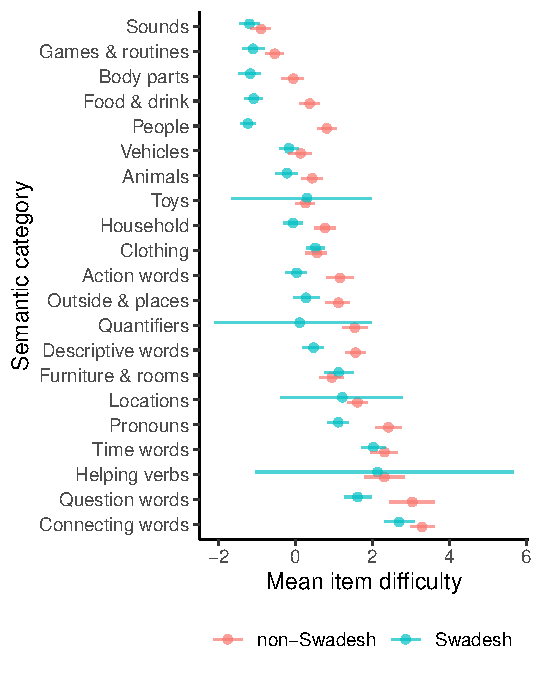
\includegraphics[keepaspectratio]{figs/fig-cat-diffs-1.pdf}}

}

\caption{\label{fig-cat-diffs}Mean cross-linguistic difficulty of CDI
words by semantic category, showing that selection of Swadesh concepts
broadly maintained representative difficulty. Bars represent
bootstrapped 95\% confidence intervals.}

\end{figure}%

Figure~\ref{fig-cat-diffs} shows the average cross-linguistic difficulty
of CDI items by semantic category, for both Swadesh and non-Swadesh
items. The difficulty of Swadesh-CDI items generally tracked with that
of non-Swadesh items.

\begin{figure}

\centering{

\pandocbounded{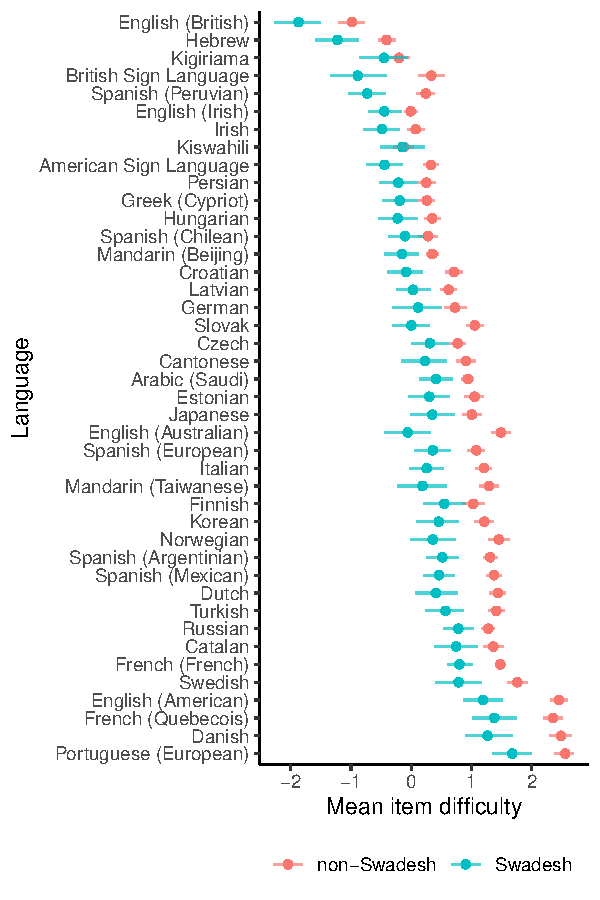
\includegraphics[keepaspectratio]{figs/fig-scdi-diffs-1.pdf}}

}

\caption{\label{fig-scdi-diffs}Mean item difficulty of Swadesh
vs.~non-Swadesh CDI items per language. Swadesh items are consistently
easier than non-Swadesh items, but show the same difficulty trend as
non-Swadesh items across languages. Bars represent bootstrapped 95\%
confidence intervals.}

\end{figure}%

Comparing the IRT parameters (across all CDI forms) showed that the
discrimination parameter (i.e., slope) of the S-CDI items did not
significantly differ from that of the non-Swadesh items, suggesting that
the S-CDI items could measure ability as well as non-Swadesh items.
However, as shown in Figure~\ref{fig-scdi-diffs}, S-CDI items were
significantly easier than the non-Swadesh items (mean S-CDI \(d=\) 0.18,
mean non-S-CDI \(d=\) 0.94, \(t(6580) = -24.68\), \(p < .001\)), which
could result in older/more-skilled children being at ceiling on the
test.

To mitigate the likelihood of a ceiling effect, we propose extending the
S-CDI with 10 additional low-variability unilemmas chosen to fill
unrepresented semantic cagegories in the S-CDI, including a helping verb
(``try''), locatives (``under'', ``in'', ``out''), quantifiers (``a
lot'', ``all'', ``many'', ``not''), and toys (``glue'', ``toy''). These
unilemmas are included on a mean of 27.5 of the 32 languages, but are of
greater difficulty (mean \(d=\) 1.14), and cross-linguistic variability
(mean \(SD(d)=\) 1.35). Adding these items forms the 110-item Swadesh
CDI Extended (S-CDI-E) list.

One additional note is that, although the S-CDI was selected on the
basis of low cross-linguistic variability in item difficulty, the S-CDI
items nonetheless showed some variability across languages (\(SD(\) mean
\(d)=\) 0.68). The deviance in mean item difficulty across languages
generally tracked with non-S-CDI items, suggesting an overall
distribution shift in the difficulty of items in the CDIs of different
languages; such shifts may be due to different sampling strategies and
age distributions of the CDI administrations in Wordbank.

\subsection{Validating the Swadesh
CDI}\label{validating-the-swadesh-cdi}

To validate the S-CDI, we first measured how well simulated raw scores
from the S-CDI items correlated with full CDI:WS scores. This metric
approximately reflects how valid the S-CDI would be as a measure of a
child's vocabulary. On average, for the 32 large CDI:WS datasets, the
S-CDI's scores were strongly related to the full CDI:WS scores (mean
\(r=0.996\); min \(=0.989\), max \(=0.998\)). We compared these
correlations against a baseline that simulated an upper bound for how
well the Swadesh CDI could be expected to perform: randomly sample \(N\)
items from the actual CDI:WS of the target language, where \(N\) is the
number of Swadesh items that are present on the form. On average, the 32
CDI forms included \(N=98\) of the Swadesh items.

Scores from a random subsample of CDI items tend to perform very well at
predicting the overall CDI score, as there are no sampling biases
related to item difficulty, or cross-linguistic variability in
difficulty or inclusion. However, note that this is \emph{not} a viable
method to create a new CDI, as in a true CDI construction scenario
rather than a simulation, the target CDI would not actually exist to
sample from! Thus, if the S-CDI comes close to performing as well as a
random sample from manually curated CDIs, we consider it a success.
Indeed, the random tests had a mean correlation with full CDI scores of
\(r=0.997\), only \(\epsilon=0.001\) higher than the S-CDI.

\subsection{Testing generalization of the Swadesh
CDI}\label{testing-generalization-of-the-swadesh-cdi}

We then evaluated the S-CDI's performance in a test of generalization to
10 more CDI datasets. For the 10 low-data languages, a comparison of
simulated S-CDI scores to full CDI:WS revealed that the S-CDI's raw
scores were again strongly related (mean \(r=0.975\)), with an average
of \(N=87.4\) S-CDI items appearing per list.
Table~\ref{tbl-gen-results} shows the results of this comparison,
alongside the upper bound random baseline. Once again, the S-CDI
performed approximately as well as a random sample of the actual CDI
(random mean \(r=0.966\)). The correlation for the 110-item S-CDI-E rose
to mean \(r=0.976\) (mean items per language: \(N=94.5\)), demonstrating
the value of including items from the more difficult semantic categories
that were underrepresented on the original list.

\begin{table}

\caption{\label{tbl-gen-results}Generalization test results, showing the
correlation between the S-CDI and the full CDI:WS sumscores.}

\centering{

\fontsize{8.2pt}{9.9pt}\selectfont
\begin{tabular*}{\linewidth}{@{\extracolsep{\fill}}lrrrrrr}
\toprule
Language & S-CDI 110 & syntactic & 2 strata & unstratified & category & random \\ 
\midrule\addlinespace[2.5pt]
American Sign Language & 0.978 & 0.976 & 0.975 & 0.974 & 0.982 & 0.984 \\ 
British Sign Language & 0.990 & 0.990 & 0.989 & 0.989 & 0.989 & 0.991 \\ 
English (Irish) & 0.968 & 0.964 & 0.974 & 0.967 & 0.973 & 0.976 \\ 
Greek (Cypriot) & 0.987 & 0.985 & 0.979 & 0.979 & 0.991 & 0.988 \\ 
Irish & 0.983 & 0.980 & 0.977 & 0.974 & 0.988 & 0.985 \\ 
Kigiriama & 0.962 & 0.964 & 0.965 & 0.962 & 0.934 & 0.932 \\ 
Kiswahili & 0.986 & 0.985 & 0.979 & 0.976 & 0.988 & 0.980 \\ 
Persian & 0.957 & 0.957 & 0.954 & 0.958 & 0.955 & 0.948 \\ 
Spanish (Chilean) & 0.970 & 0.968 & 0.966 & 0.969 & 0.900 & 0.907 \\ 
Spanish (Peruvian) & 0.983 & 0.980 & 0.979 & 0.957 & 0.956 & 0.966 \\ 
\midrule
{Mean} & {0.976} & {0.975} & {0.974} & {0.970} & {0.966} & {0.966} \\ 
\bottomrule
\end{tabular*}

}

\end{table}%

\section{Discussion}\label{discussion}

Assessing early language development is important in all language
communities. However, it is difficult to adapt existing measures such as
the CDI to understudied languages, especially with the goal of enabling
cross-linguistic comparisons of early learning. This study leveraged
psychometric models fitted to 32 CDI datasets in order to find concepts
that had low variability in their cross-linguistic difficulty and that
were frequently included on CDI forms. This analysis identified 100
concepts that appeared on at least 27 of the CDIs and which had more
consistent cross-linguistic difficulty than other concepts appearing on
multiple CDIs. Using real-data simulations, we showed that administering
this set of Swadesh CDI items would generate children's production
vocabulary scores that were strongly related to full CDI scores, both
for the original 32 datasets, and in a generalization test to 10
low-data languages. Moreover, the S-CDI items resulted in comparable
performance to tests of the same length composed of randomly-selected
unilemmas from the target test---a challenging baseline to beat and a
construction method impossible to use when creating a new CDI. The S-CDI
contains items with relatively stable cross-linguistic difficulty
estimates and, in the absence of researchers who are familiar with
relevant local cultures and concepts, they may serve as a rapid, simple
means of approximating children's ability levels, even when a large
norming dataset is not available. Additionally, the S-CDI items also
overlapped with other common 100-word lists used in lexicostatistics,
vocabulary assessment, and pedagogy, as shown in the Appendix.

It is notable that, regardless of our stratification procedure, the
number of selected overlapping items and the cross-validated difficulty
correlations were both relatively high. In other words, a fairly large
number of items had similar difficulties across languages, meaning that
they are acquired at similar ages. This result corroborates and extends
previous findings from Tardif et al. (2008) and Frank et al. (2021), who
found substantial consistency in children's early vocabularies across
languages. As in Frank et al. (2021), we also found that the S-CDI items
were easier than other items in general, suggesting that
earlier-acquired vocabulary items are more consistent than later ones.
Furthermore, it is interesting to observe the distribution of
Swadesh-CDI items across semantic categories; notably, our final list
underrepresented toys, food and drink, and things found outside, all of
which may be more culturally contingent, and thus more variable than
other categories. Similarly the S-CDI also underrepresented quantifiers,
auxiliary verbs, and locatives, which are grammatical items that may
exhibit more cross-linguistic variability than other categories. The
distribution of S-CDI items supports the idea that early vocabularies
are conditioned both on broad similarities in early childhood
experience, as well as cultural and linguistic differences in accessible
concepts and words.

As previously mentioned, the S-CDI items were significantly easier than
other items, meaning that older children may perform at ceiling if given
only the S-CDI items. (This may be unsurprising from the perspective
that Swadesh words are meant to be universal, and are therefore more
frequent and basic---both within and across individual children's
experiences.) Thus, our suggested use case for the S-CDI list is as a
starting point for researchers seeking to develop a CDI in a new
language, rather than as a complete short-form CDI based on existing
long-form CDI data. In particular, researchers should seek to add
relevant unilemmas relevant for the new language from categories that
are less well-represented on the S-CDI, including helping verbs,
locatives, quantifiers, and toys. These categories also tended to be
more difficult, so adding items from them is likely to increase the
difficulty of the form and limit ceiling effects. Indeed, the inclusion
of 10 low-variability items in the S-CDE-E representing these missing
semantic categories increased generalization performance. Researchers
adapting the S-CDI to new languages should also consider replacing nouns
that may be less appropriate in some contexts (e.g.~``TV'', ``washing machine'',
``elephant'', ``dog'').

Another potential limitation of this work is that most existing CDIs
(and most datasets available in Wordbank) target languages in the
Indo-European language family. It is not clear to what extent this bias
in the existing data might interfere with generalizing to
non-Indo-European languages. Nonetheless, our original 32 datasets
include 11 non-Indo-European languages (3 Sino-Tibetan, 3 Uralic, 2
Afro-Asiatic, 1 Japonic, 1 Koreanic, 1 Turkic), and the generalization
datasets include 2 sign languages and 2 Niger-Congo languages, two
language families not represented in the original datasets; the broad
consistency across language families thus suggests that the
effectiveness of the S-CDI may be sufficiently robust. Such a robustness
also corroborates with results from Floccia et al. (2018), who
demonstrated that a bilingual vocabulary model based on a set of 30
unilemmas had good predictive validity on non-target languages, even
those from other language families.

Developing a list of appropriate vocabulary words is not the only
challenge researchers face when seeking to develop and use parent-report
measures in a new language and culture. The pragmatics of language
between children and adults can differ greatly across cultures, and has
been found to interfere with administration of parent-report measures of
early vocabulary, for example in Kiswahili (Alcock 2017) and Wolof
(Weber et al. 2018), where the variety and amount of infant-directed
speech differs from Western contexts (see Bergelson et al. 2023; Bunce
et al. 2024). As such, local cultural knowledge remains essential to
consider to assure appropriate development of CDI adaptations.

Contexts in which children are learning more than one language
simultaneously present another obstacle in the creation of a universal
CDI, as cultural knowledge is needed to adjudicate which concepts and
translation equivalents are appropriate for inclusion. The psychometric
approach used for the S-CDI generalizes the method used to develop the
DLL EN-ES (Tamis-LeMonda 2024), a measure intended for English--Spanish
bilingual language learners. Developing those instruments involved an
iterative process of identifying translation-equivalent items with large
discrepancy in cross-linguistic (English vs.~Spanish) difficulty (e.g.,
``hat'' and ``sombrero''), and replacing them with CDI items that were
appropriate in both languages (informed by researchers with local
knowledge), and had minimal difference in cross-linguistic difficulty.
We strongly recommend that the S-CDI list serve only as a starting point
for developing a new CDI, and that researchers also use an iterative
process that takes into account local expert knowledge of the target
language, as well as the potential for multilingual learning contexts in
order to select appropriate items. While keeping these limitations and
considerations in mind, here we propose a procedure for developing a
Swadesh-based CDI.

\subsection{Guide to developing a Swadesh-based
CDI}\label{guide-to-developing-a-swadesh-based-cdi}

Developing a CDI for a new language is a substantial task requiring
specific linguistic and cultural knowledge---even with the new
Swadesh-CDI recommendations in hand. Many recommendations and caveats
have been enumerated by the CDI Advisory Board,\footnote{The adaptation 
guidelines can be found at \url{https://mb-cdi.stanford.edu/adaptations.html}}
and Jarůšková et al. (2023) also present a comprehensive guide to
adapting the CDI to new languages. Rather than recapitulate the
processes and caveats already itemized in those resources, we suggest
how the Swadesh CDI can be used to jump-start the process.

\begin{enumerate}
\def\labelenumi{\arabic{enumi}.}
\tightlist
\item
  As a starting point, take the 100 S-CDI unilemmas, and consider their
  linguistic and cultural appropriateness for the target language.
  Include as many as are relevant.
\item
  Consider adding unilemmas that are frequently included on other CDIs,
  and especially focus on semantic categories that are less
  well-represented on the S-CDI, including helping verbs, quantifiers,
  locatives, and toys. We recommend adding 10--20 items across these
  categories, including the 10-item extension we tested, which are
  present on many existing CDI forms (``try'', ``under'', ``in'',
  ``out'', ``a lot'', ``all'', ``many'', ``not'', ``glue (object)'',
  ``toy'').
\item
  Do a pilot study, including several children at the upper and lower
  intended ages, and revise if there are many children at floor or
  ceiling.
\end{enumerate}

\subsection{Conclusion}\label{conclusion}

Despite the myriad challenges that remain in creating new measures of
early language development, we believe that the proposed Swadesh CDI
list will give researchers a solid foundation from which to start,
lowering the barrier to the adaptation of CDI forms in new languages,
since these are often time-consuming and challenging to construct.
Expanding the number of languages with effective vocabulary measures
would be a critical step in addressing issues related to the
under-representation of linguistic diversity in language acquisition
research (Kidd and Garcia 2022). Certainly, increasing the diversity of
languages studied is a critical step towards developing a truly general
understanding of how young children learn language.

\section{Acknowledgements}\label{acknowledgements}

We would like to thank all of the contributors to Wordbank, from the
researchers who created and adapted the CDIs to those who collected the
data as well as all participants.

\section{References}\label{references}

\phantomsection\label{refs}
\begin{CSLReferences}{1}{0}
\bibitem[\citeproctext]{ref-alcock2017production}
Alcock, Katherine J. 2017. {``Production Is Only Half the Story---First
Words in Two {East African} Languages.''} \emph{Frontiers in Psychology}
8: 1898.

\bibitem[\citeproctext]{ref-Baker2001}
Baker, Frank B. 2001. \emph{The Basics of Item Response Theory}. ERIC.

\bibitem[\citeproctext]{ref-bates1994}
Bates, Elizabeth, Virginia Marchman, Donna Thal, Larry Fenson, Philip S
Dale, J Steven Reznick, Judy Reilly, and Jeff Hartung. 1994.
{``Developmental and Stylistic Variation in the Composition of Early
Vocabulary.''} \emph{Journal of Child Language} 21 (1): 85--123.

\bibitem[\citeproctext]{ref-bergelson2023}
Bergelson, Elika, Melanie Soderstrom, Iris-Corinna Schwarz, Caroline F.
Rowland, Nairán Ramírez-Esparza, Lisa R. Hamrick, Ellen Marklund, et al.
2023. {``Everyday Language Input and Production in 1,001 Children from
Six Continents.''} \emph{Proceedings of the National Academy of
Sciences} 120 (52). \url{https://doi.org/10.1073/pnas.2300671120}.

\bibitem[\citeproctext]{ref-bleses2016}
Bleses, Dorthe, Guido Makransky, Philip S Dale, Anders Højen, and Burcak
Aktürk Ari. 2016. {``Early Productive Vocabulary Predicts Academic
Achievement 10 Years Later.''} \emph{Applied Psycholinguistics} 37 (6):
1461--76.

\bibitem[\citeproctext]{ref-brookes2025}
Brookes, Heather, Frenette Southwood, Martin Mössmer, Patricia Makaure,
Michelle White, Carmen Defty, Sefela Yalala, et al. 2025. {``Instrument
Adaptation for Measuring Early Child Language Development Across
Multilingual and Sociocultural Diverse Settings''} Online First
Publication (February). \url{https://doi.org/10.1037/dev0001935}.

\bibitem[\citeproctext]{ref-bunce2024}
Bunce, John, Melanie Soderstrom, Elika Bergelson, Celia Rosemberg,
Alejandra Stein, Florencia Alam, Maia Julieta Migdalek, and Marisa
Casillas. 2024. {``A Cross-Linguistic Examination of Young Children's
Everyday Language Experiences.''} \emph{Journal of Child Language} 52
(4): 786--814. \url{https://doi.org/10.1017/s030500092400028x}.

\bibitem[\citeproctext]{ref-chai2020}
Chai, Jun Ho, Chang Huan Lo, and Julien Mayor. 2020. {``A
{B}ayesian-Inspired Item Response Theory-Based Framework to Produce Very
Short Versions of {M}ac{A}rthur-{B}ates {C}ommunicative {D}evelopment
{I}nventories.''} \emph{Journal of Speech, Language, and Hearing
Research} 63 (10): 3488--3500.

\bibitem[\citeproctext]{ref-R-mirt}
Chalmers, R. Philip. 2012. {``{mirt}: A Multidimensional Item Response
Theory Package for the {R} Environment.''} \emph{Journal of Statistical
Software} 48 (6): 1--29. \url{https://doi.org/10.18637/jss.v048.i06}.

\bibitem[\citeproctext]{ref-eberhard2025}
Eberhard, David M., Gary F. Simons, and Charles D. Fennig, eds. 2025.
\emph{Ethnologue: Languages of the World}. 28th ed. Dallas, TX: SIL
International.

\bibitem[\citeproctext]{ref-embretson2013}
Embretson, Susan E, and Steven P Reise. 2013. \emph{Item Response
Theory}. Psychology Press.

\bibitem[\citeproctext]{ref-Fenson2007}
Fenson, Larry, V. A. Marchman, D. J. Thal, P. S. Dale, Reznick J. S.,
and E. Bates. 2007. \emph{{M}ac{A}rthur-{B}ates {C}ommunicative
{D}evelopment {I}nventories: User's Guide and Technical Manual (2nd
Ed.)}. Baltimore, MD: Brookes.

\bibitem[\citeproctext]{ref-floccia2018vocabulary}
Floccia, Caroline, Thomas D Sambrook, Claire Delle Luche, Rosa Kwok,
Jeremy Goslin, Laurence White, Allegra Cattani, et al. 2018.
{``Vocabulary of 2-Year-Olds Learning Learning English and an Additional
Language: Norms and Effects of Linguistic Distance.''}

\bibitem[\citeproctext]{ref-frank2017}
Frank, Michael C, Mika Braginsky, Daniel Yurovsky, and Virginia A
Marchman. 2017. {``Wordbank: An Open Repository for Developmental
Vocabulary Data.''} \emph{Journal of Child Language} 44 (3): 677.

\bibitem[\citeproctext]{ref-frank2021}
---------. 2021. \emph{Variability and Consistency in Early Language
Learning: The {Wordbank} Project}. MIT Press.

\bibitem[\citeproctext]{ref-fry1980}
Fry, E. 1980. {``The New Instant Word List.''} \emph{The Reading
Teacher} 34 (3): 284--89.

\bibitem[\citeproctext]{ref-green2024}
Green, Clarence, Kathleen Keogh, and Julia Prout. 2024. {``The {CPB}
Sight Words: A New Research‐based High‐frequency Wordlist for Early
Reading Instruction.''} \emph{The Reading Teacher} 78 (1): 56--64.

\bibitem[\citeproctext]{ref-hamilton2000}
Hamilton, A, K Plunkett, and G Schafer. 2000. {``Infant Vocabulary
Development Assessed with a British Communicative Development
Inventory.''} \emph{Journal of Child Language} 27 (3): 689--705.

\bibitem[\citeproctext]{ref-hellwig2021}
Hellwig, Birgit, Rebecca Defina, Evan Kidd, Shanley E M Allen, Lucinda
Davidson, and Barbara F Kelly. 2021. {``Child Language Documentation:
{The} Sketch Acquisition Project.''} In \emph{Doing Corpus-Based
Typology with Spoken Language Data: {State} of the Art}, edited by
Geoffrey Haig, Stefan Schnell, and Frank Seifart, 29--58. Language
{Documentation} \& {Conservation Special Publication} 25. Honolulu, HI:
University of Hawai'i Press.

\bibitem[\citeproctext]{ref-jaruskova2023}
Jarůšková, Lucie, Filip Smolík, Kateřina Chládková, Zuzana Oceláková,
and Nikola Paillereau. 2023. {``How to {Build} a {Communicative
Development Inventory}: {Insights From} 43 {Adaptations}.''}
\emph{Journal of Speech, Language, and Hearing Research}.
\url{https://doi.org/10.1044/2023_JSLHR-22-00591}.

\bibitem[\citeproctext]{ref-Kachergis2022}
Kachergis, G., V. A. Marchman, P. S. Dale, J. Mankewitz, and M. C.
Frank. 2022. {``Online Computerized Adaptive Tests of Children's
Vocabulary Development in {English} and {Mexican Spanish}.''}
\emph{Journal of Speech, Language, and Hearing Research} 65 (6):
2288--308.

\bibitem[\citeproctext]{ref-kidd2022}
Kidd, Evan, and Rowena Garcia. 2022. {``How Diverse Is Child Language
Acquisition Research?''} \emph{First Language} 42 (6): 703--35.
\url{https://doi.org/10.1177/01427237211066405}.

\bibitem[\citeproctext]{ref-Makransky2016}
Makransky, G., P. S. Dale, P. Havmose, and D. Bleses. 2016. {``An Item
Response Theory-Based, Computerized Adaptive Testing Version of the
{M}ac{A}rthur-{B}ates {C}ommunicative {D}evelopment {I}nventory: {W}ords
\& {S}entences ({CDI:WS}).''} \emph{Journal of Speech, Language, and
Hearing Research} 59 (2): 281--89.

\bibitem[\citeproctext]{ref-marchman2023}
Marchman, Virginia A, Philip S Dale, and Larry Fenson. 2023.
\emph{MacArthur-Bates Communicative Development Inventories User's Guide
and Technical Manual, 3rd Edition}. Baltimore, MD: Brookes Publishing
Co.

\bibitem[\citeproctext]{ref-mayor2019}
Mayor, Julien, and Nivedita Mani. 2019. {``A Short Version of the
{M}ac{A}rthur-{B}ates {C}ommunicative {D}evelopment {I}nventories with
High Validity.''} \emph{Behavior Research Methods} 51 (5): 2248--55.

\bibitem[\citeproctext]{ref-singh2023}
Singh, Leher, Alejandrina Cristia, Lana B. Karasik, Sarah J. Rajendra,
and Lisa M. Oakes. 2023. {``Diversity and Representation in Infant
Research: {Barriers} and Bridges Toward a Globalized Science of Infant
Development.''} \emph{Infancy} 28 (4): 708--37.
\url{https://doi.org/10.1111/infa.12545}.

\bibitem[\citeproctext]{ref-Swadesh1971}
Swadesh, M. 1971. \emph{The Origin and Diversification of Language}.
Edited by Joel Sherzer. Chicago, IL: Aldine.

\bibitem[\citeproctext]{ref-tadmor2010}
Tadmor, Uri, Martin Haspelmath, and Bradley Taylor. 2010.
{``Borrowability and the Notion of Basic Vocabulary.''}
\emph{Diachronica} 27 (2): 226--46.

\bibitem[\citeproctext]{ref-tamislemonda2024dll}
Tamis-LeMonda, Kachergis, C. S. 2024. {``Comparing Apples to Manzanas
and Oranges to Naranjas: A New Measure of English-Spanish Vocabulary for
Dual Language Learners.''} \emph{Infancy} 29.
\url{https://doi.org/10.1111/infa.12571}.

\bibitem[\citeproctext]{ref-tardif2008baby}
Tardif, Twila, Paul Fletcher, Weilan Liang, Zhixiang Zhang, Niko
Kaciroti, and Virginia A Marchman. 2008. {``Baby's First 10 Words.''}
\emph{Developmental Psychology} 44 (4): 929.

\bibitem[\citeproctext]{ref-weber2018}
Weber, Ann M., Virginia A. Marchman, Yatma Diop, and Anne Fernald. 2018.
{``Validity of Caregiver-Report Measures of Language Skill for
{Wolof}-Learning Infants and Toddlers Living in Rural African
Villages.''} \emph{Journal of Child Language} 45 (4): 939--58.
\url{https://doi.org/10.1017/S0305000917000605}.

\end{CSLReferences}

\section{Additional detailed methods and
results}\label{additional-detailed-methods-and-results}

\subsection{Unilemma operationalisation and
updating}\label{unilemma-operationalisation-and-updating}

Unilemmas are rough cross-linguistic conceptual mappings for words. For
example, ``dog'' (English), ``perro'' (Spanish), and ``chien'' (French)
all seem like they describe the same concept, \emph{dog}. We thus have
\emph{dog} as the unilemma for this concept, allowing mapping between
different forms in different languages.

Decisions about which words correspond to which unilemmas are
necessarily somewhat arbitrary. Our design intention for unilemmas was
to provide reasonable mappings, lumping together many meanings rather
than splitting them, allowing us to build predictive models of
cross-linguistic similarities and differences in acquisition. If we
split the conceptual world too finely, it would be difficult to
understand how similar the information sources are; if we split too
coarsely, we can at least discover that languages differ by the
differences in predictors.

However, we also preserve distinctions for concepts that are \emph{prima
facie} similar, but that play very different cultural roles. For
example, although ``pan'' (Spanish) and ``tortilla'' (Mexican Spanish)
are relatively similar, they play different cultural roles in Mexican
Spanish, and hence we err towards splitting these into separate
categories.

There remained other issues regarding unilemma definitions, including
cases of polysemy, handling syntactic categories, and pronouns; in each
case, we made decisions based on our best guess of the most basic or
common interpretation in the child language context. Further details can
be found in our unilemma policy document, available at
\url{https://github.com/langcog/update_unilemmas/blob/main/unilemma_policy.md}.

We then recruited native or advanced proficient speakers of all the
languages in Wordbank to help verify and correct unilemmas for the CDI
forms. Subsequently, two of the authors (GK, AWMT) reviewed the
suggestions and made decisions about conflicts, and standardized
unilemmas into a canonical form across all instruments. More details
about the recent update can be found at
\url{https://github.com/langcog/update_unilemmas}.

\subsection{Cross-validation results}\label{cross-validation-results-1}

\begin{figure}[ht]

\centering{

\pandocbounded{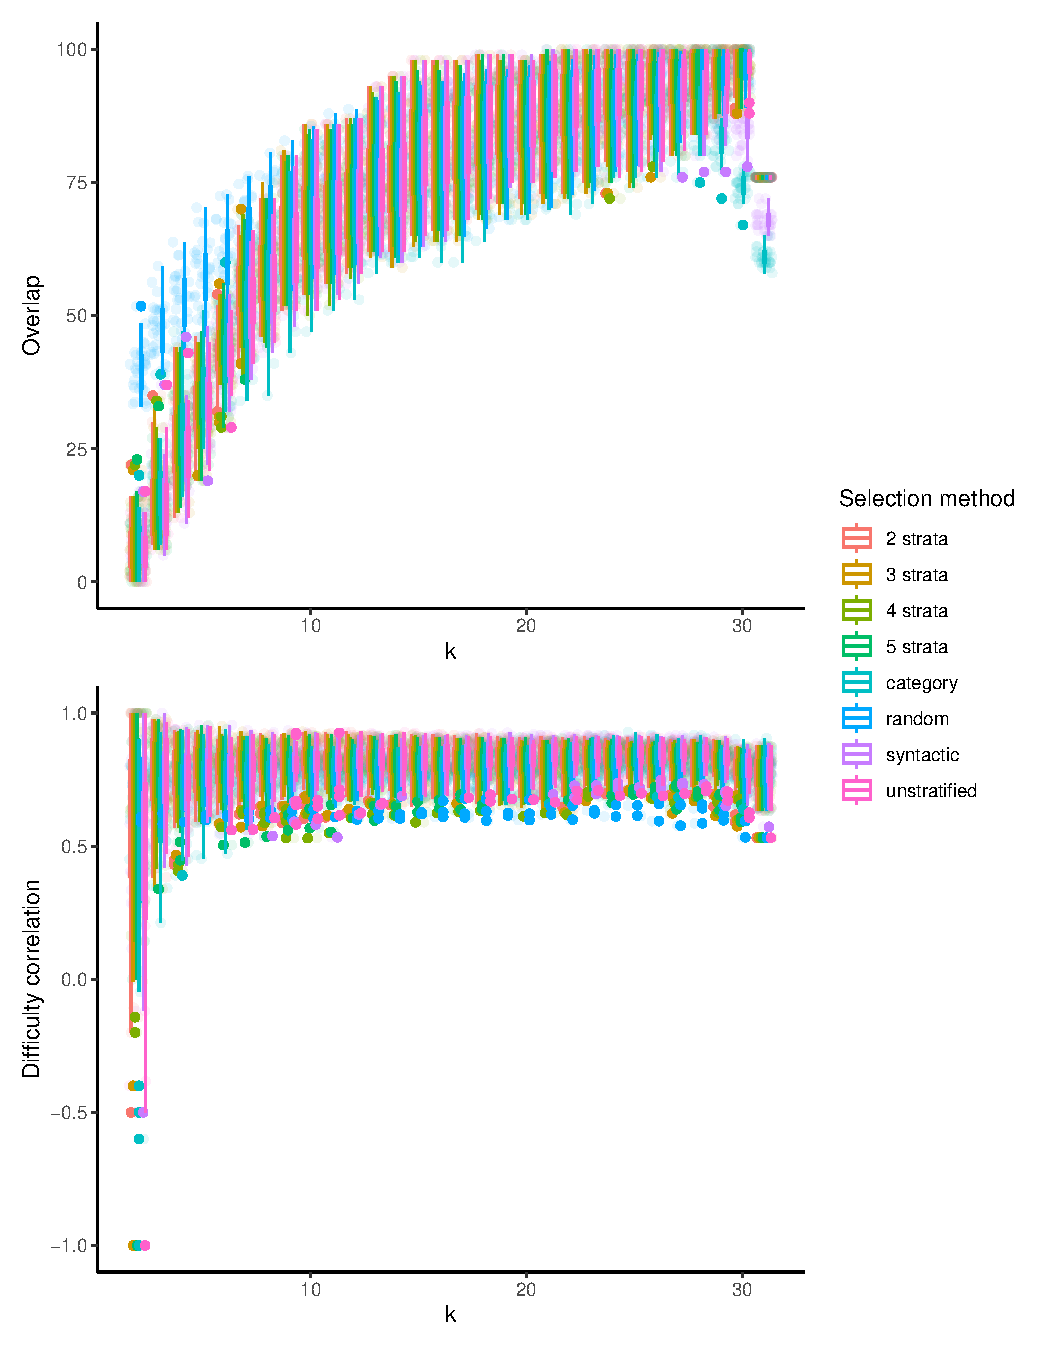
\includegraphics[keepaspectratio]{figs/fig-cv-1.pdf}}

}

\caption{\label{fig-cv}Difficulty correlation and overlap by k for the
different sublist selection methods.}

\end{figure}%

Figure~\ref{fig-cv} shows the full cross-validation results for the
different sublist selection methods, showing the number of overlapping
items and item-wise correlations in difficulty as a function of \(k\),
the minimum number of languages in which the items appear.

\subsection{Swadesh CDI vs.~full
CDI:WS}\label{swadesh-cdi-vs.-full-cdiws}

Table~\ref{tbl-full-correl} shows the correlation between the sumscores
of the full CDI and Swadesh-CDI for syntactic category stratification
method, for items on at least \(k=27\) CDIs, for each of the 32
languages that the IRT models were trained on.

\begin{table}[ht]

\caption{\label{tbl-full-correl}Sumscore correlations between S-CDI and
full CDI:WS for 32 training languages.}

\centering{

\fontsize{12.0pt}{14.4pt}\selectfont
\begin{tabular*}{\linewidth}{@{\extracolsep{\fill}}lrr}
\toprule
Language & Overlap & Sumscore \(r\) \\ 
\midrule\addlinespace[2.5pt]
Arabic (Saudi) & 95 & 0.966 \\ 
Cantonese & 90 & 0.986 \\ 
Catalan & 93 & 0.989 \\ 
Croatian & 97 & 0.992 \\ 
Czech & 94 & 0.988 \\ 
Danish & 99 & 0.992 \\ 
Dutch & 98 & 0.965 \\ 
English (American) & 98 & 0.989 \\ 
English (Australian) & 76 & 0.990 \\ 
English (British) & 90 & 0.929 \\ 
Estonian & 93 & 0.990 \\ 
Finnish & 95 & 0.944 \\ 
French (French) & 97 & 0.973 \\ 
French (Quebecois) & 98 & 0.985 \\ 
German & 90 & 0.991 \\ 
Hebrew & 87 & 0.980 \\ 
Hungarian & 96 & 0.989 \\ 
Italian & 97 & 0.991 \\ 
Japanese & 86 & 0.986 \\ 
Korean & 87 & 0.986 \\ 
Latvian & 96 & 0.989 \\ 
Mandarin (Beijing) & 92 & 0.988 \\ 
Mandarin (Taiwanese) & 88 & 0.991 \\ 
Norwegian & 97 & 0.992 \\ 
Portuguese (European) & 91 & 0.988 \\ 
Russian & 89 & 0.987 \\ 
Slovak & 84 & 0.988 \\ 
Spanish (Argentinian) & 96 & 0.984 \\ 
Spanish (European) & 84 & 0.986 \\ 
Spanish (Mexican) & 94 & 0.988 \\ 
Swedish & 96 & 0.985 \\ 
Turkish & 87 & 0.990 \\ 
\bottomrule
\end{tabular*}

}

\end{table}%

\subsection{Comparison of Swadesh CDI items to other
lists}\label{comparison-of-swadesh-cdi-items-to-other-lists}

There are several short vocabulary lists of 100 items that have been
constructed for different purposes, which serve as useful comparisons to
the Swadesh CDI list. In Table~\ref{tbl-form-compare}, we list the items
on the S-CDI list, and whether they also occur in other short vocabulary
lists. We considered two lists used in lexicostatistics: the original
Swadesh-100 list (Swadesh 1971) and the Leipzig--Jakarta list (Tadmor,
Haspelmath, and Taylor 2010). We also included three short form CDI
lists used for vocabulary assessment: the American English CDI:WS Short
Forms A and B (Marchman, Dale, and Fenson 2023), and the Oxford Short
Form (Hamilton, Plunkett, and Schafer 2000). Finally, we included two
lists used for pedagogical instruction: the Fry-100 Sight Words list
(Fry 1980), and the Children's Picture Book Sight Words list (Green,
Keogh, and Prout 2024). These lists range in overlap with the S-CDI,
from 13 items (Fry-100 and Children's Picture Book) to 25 items (Oxford
Short Form CDI); the overlap in items suggests that the S-CDI list
captures some of the relevant dimensions of early vocabulary
(consistency across languages, utility in assessment, and pedagogical
importance).

\begingroup
\setlength\LTleft{0\linewidth}
\setlength\LTright{0\linewidth}\fontsize{7.5pt}{9.0pt}\selectfont

\begin{longtable}{@{\extracolsep{\fill}}>{\raggedright\arraybackslash}p{\dimexpr 80.25pt -2\tabcolsep-1.5\arrayrulewidth}>{\raggedright\arraybackslash\everypar{\hangindent=1em}}p{\dimexpr 60.00pt -2\tabcolsep-1.5\arrayrulewidth}>{\centering\arraybackslash}p{\dimexpr 45.00pt -2\tabcolsep-1.5\arrayrulewidth}>{\centering\arraybackslash}p{\dimexpr 45.00pt -2\tabcolsep-1.5\arrayrulewidth}>{\centering\arraybackslash}p{\dimexpr 45.00pt -2\tabcolsep-1.5\arrayrulewidth}>{\centering\arraybackslash}p{\dimexpr 45.00pt -2\tabcolsep-1.5\arrayrulewidth}>{\centering\arraybackslash}p{\dimexpr 45.00pt -2\tabcolsep-1.5\arrayrulewidth}>{\centering\arraybackslash}p{\dimexpr 45.00pt -2\tabcolsep-1.5\arrayrulewidth}>{\centering\arraybackslash}p{\dimexpr 45.00pt -2\tabcolsep-1.5\arrayrulewidth}}

\caption{\label{tbl-form-compare}Comparison of the S-CDI list with other
100-item vocabulary lists. Italicized words are in the S-CDI-E 10-item extension. 
SF: Short form. CPB: Children's Picture Book}

\tabularnewline

\toprule
 &  & \multicolumn{2}{>{\centering\arraybackslash}m{\dimexpr 90.00pt -2\tabcolsep-1.5\arrayrulewidth}}{Lexicostatistics} & \multicolumn{3}{>{\centering\arraybackslash}m{\dimexpr 135.00pt -2\tabcolsep-1.5\arrayrulewidth}}{Assessment} & \multicolumn{2}{>{\centering\arraybackslash}m{\dimexpr 90.00pt -2\tabcolsep-1.5\arrayrulewidth}}{Pedagogy} \\ 
\cmidrule(lr){3-4} \cmidrule(lr){5-7} \cmidrule(lr){8-9}
Semantic category & S-CDI items & Original Swadesh list & Leipzig– Jakarta list & CDI:WS SF A & CDI:WS SF B & Oxford SF CDI & Fry Sight Words & CPB Sight Words \\ 
\midrule\addlinespace[2.5pt]
Actions & blow &  & Y &  &  &  &  &  \\ 
 & cry &  & Y &  &  &  &  &  \\ 
 & dance &  &  &  &  &  &  &  \\ 
 & eat & Y & Y &  &  &  &  &  \\ 
 & fall &  & Y &  &  & Y &  &  \\ 
 & help &  &  &  &  &  &  &  \\ 
 & jump &  &  &  & Y &  &  &  \\ 
 & push &  &  &  &  &  &  &  \\ 
 & sing &  &  &  &  &  &  &  \\ 
 & sit & Y &  &  & Y &  &  &  \\ 
 & wait &  &  &  &  &  &  &  \\ 
Animals & animal &  &  &  &  &  &  &  \\ 
 & ant &  & Y &  &  &  &  &  \\ 
 & bee &  &  &  &  &  &  &  \\ 
 & cat &  &  & Y &  &  &  &  \\ 
 & cow &  &  &  &  &  &  &  \\ 
 & dog & Y & Y & Y &  &  &  &  \\ 
 & elephant &  &  &  &  & Y &  &  \\ 
 & horse &  &  & Y &  &  &  &  \\ 
 & lion &  &  &  &  & Y &  &  \\ 
 & monkey &  &  &  &  &  &  &  \\ 
 & owl &  &  &  &  &  &  &  \\ 
 & sheep &  &  &  &  &  &  &  \\ 
 & tiger &  &  &  &  &  &  &  \\ 
 & turtle &  &  &  &  &  &  &  \\ 
 & wolf &  &  &  &  &  &  &  \\ 
Body parts & chin &  &  & Y &  &  &  &  \\ 
 & eye & Y & Y &  &  &  &  &  \\ 
 & mouth & Y & Y &  &  & Y &  &  \\ 
 & nose & Y & Y &  & Y & Y &  &  \\ 
 & tongue & Y & Y &  & Y &  &  &  \\ 
 & tooth & Y & Y &  &  &  &  &  \\ 
Clothing & bib &  &  &  &  & Y &  &  \\ 
 & button &  &  &  &  &  &  &  \\ 
 & dress &  &  &  &  &  &  &  \\ 
Connectives & and &  &  &  &  &  & Y & Y \\ 
 & but &  &  &  &  &  & Y & Y \\ 
Descriptives & black & Y & Y &  & Y &  &  &  \\ 
 & blue &  &  &  &  &  &  &  \\ 
 & cold & Y &  & Y &  & Y &  &  \\ 
 & dirty &  &  &  & Y & Y &  &  \\ 
 & green & Y &  &  &  &  &  &  \\ 
 & heavy &  & Y &  &  &  &  &  \\ 
 & hot & Y &  & Y &  & Y &  &  \\ 
 & red & Y & Y &  &  &  &  &  \\ 
 & white & Y &  &  &  &  &  &  \\ 
 & yellow & Y &  &  &  &  &  &  \\ 
Food \& drink & banana &  &  &  &  &  &  &  \\ 
 & candy &  &  & Y &  &  &  &  \\ 
 & coffee &  &  &  &  &  &  &  \\ 
 & milk &  &  & Y &  & Y &  &  \\ 
 & yogurt &  &  &  &  &  &  &  \\ 
Furniture \& rooms & garage &  &  &  &  &  &  &  \\ 
 & TV &  &  &  &  &  &  &  \\ 
 & washing machine &  &  &  &  &  &  &  \\ 
Games \& routines & shh &  &  &  &  &  &  &  \\ 
 & yes &  &  &  &  & Y &  &  \\ 
Helping verbs & \emph{try} &  &  &  &  &  &  &  \\ 
Household & broom &  &  & Y &  & Y &  &  \\ 
 & glasses &  &  &  &  & Y &  &  \\ 
 & hammer &  &  &  &  &  &  &  \\ 
 & key &  &  &  & Y & Y &  &  \\ 
 & radio &  &  &  &  &  &  &  \\ 
 & spoon &  &  &  &  &  &  &  \\ 
 & telephone &  &  &  &  &  &  &  \\ 
 & toothbrush &  &  &  &  &  &  &  \\ 
Locations & \emph{in} &  & Y &  &  & Y & Y & Y \\ 
 & \emph{out} &  &  &  &  &  & Y & Y \\ 
 & \emph{under} &  &  & Y &  &  &  &  \\ 
Outside \& places & moon & Y &  &  &  &  &  &  \\ 
 & school &  &  & Y &  &  &  &  \\ 
People & child's own name &  &  &  &  &  &  &  \\ 
 & daddy &  &  &  &  &  &  &  \\ 
 & doctor &  &  &  &  &  &  &  \\ 
 & mommy &  &  & Y & Y & Y &  &  \\ 
 & police &  &  &  &  &  &  &  \\ 
Pronouns & 1SG (I) & Y & Y &  &  & Y & Y & Y \\ 
 & 2SG (you) & Y & Y &  &  &  & Y & Y \\ 
 & 2SG.POSS (your) &  &  &  &  &  & Y & Y \\ 
 & 3SG (he/she/it) &  & Y &  & Y & Y & Y & Y \\ 
 & that & Y &  &  &  &  & Y & Y \\ 
 & this & Y & Y & Y &  &  & Y & Y \\ 
Quantifiers & \emph{a lot} &  &  &  &  &  &  &  \\ 
 & \emph{all} & Y &  & Y &  &  & Y & Y \\ 
 & \emph{many} & Y &  &  &  &  & Y &  \\ 
 & \emph{not} & Y & Y &  &  & Y & Y & Y \\ 
Question words & how &  &  &  &  &  & Y & Y \\ 
 & what & Y & Y &  &  & Y & Y & Y \\ 
 & when &  &  &  &  &  & Y & Y \\ 
 & where &  &  & Y &  & Y &  &  \\ 
 & who & Y & Y &  &  &  & Y & Y \\ 
 & why &  &  &  & Y & Y &  &  \\ 
Sounds & baa baa &  &  & Y & Y &  &  &  \\ 
 & cockadoodledoo &  &  &  &  & Y &  &  \\ 
 & meow &  &  & Y &  &  &  &  \\ 
 & quack quack &  &  &  &  &  &  &  \\ 
 & vroom &  &  &  &  &  &  &  \\ 
 & woof woof &  &  & Y &  &  &  &  \\ 
Time words & now &  &  &  &  & Y & Y & Y \\ 
 & today &  &  &  & Y & Y &  &  \\ 
 & tomorrow &  &  &  & Y & Y &  &  \\ 
 & yesterday &  & Y &  &  &  &  &  \\ 
Toys & \emph{glue} &  &  &  &  &  &  &  \\ 
 & \emph{toy} &  &  &  &  &  &  &  \\ 
Vehicles & airplane &  &  & Y &  & Y &  &  \\ 
 & bicycle &  &  &  &  &  &  &  \\ 
 & helicopter &  &  &  &  &  &  &  \\ 
 & truck &  &  &  & Y &  &  &  \\ 
\midrule
{S-CDI overlap} & {} & {22} & {21} & {17} & {14} & {25} & {13} & {13} \\ 
S-CDI-E overlap &  & 25 & 23 & 19 & 14 & 27 & 18 & 17 \\ 
\bottomrule

\end{longtable}

\endgroup


\end{document}
